\chapter{Impact Analysis in Variation of the Buffer Size}
\label{D_Kapitel}
\noindent In this chapter we attepmt to explorer the relationship between the  paramters and the transient performance of a multi-machine line with five machines. 

\begin{figure*}[!h]
    \centering
		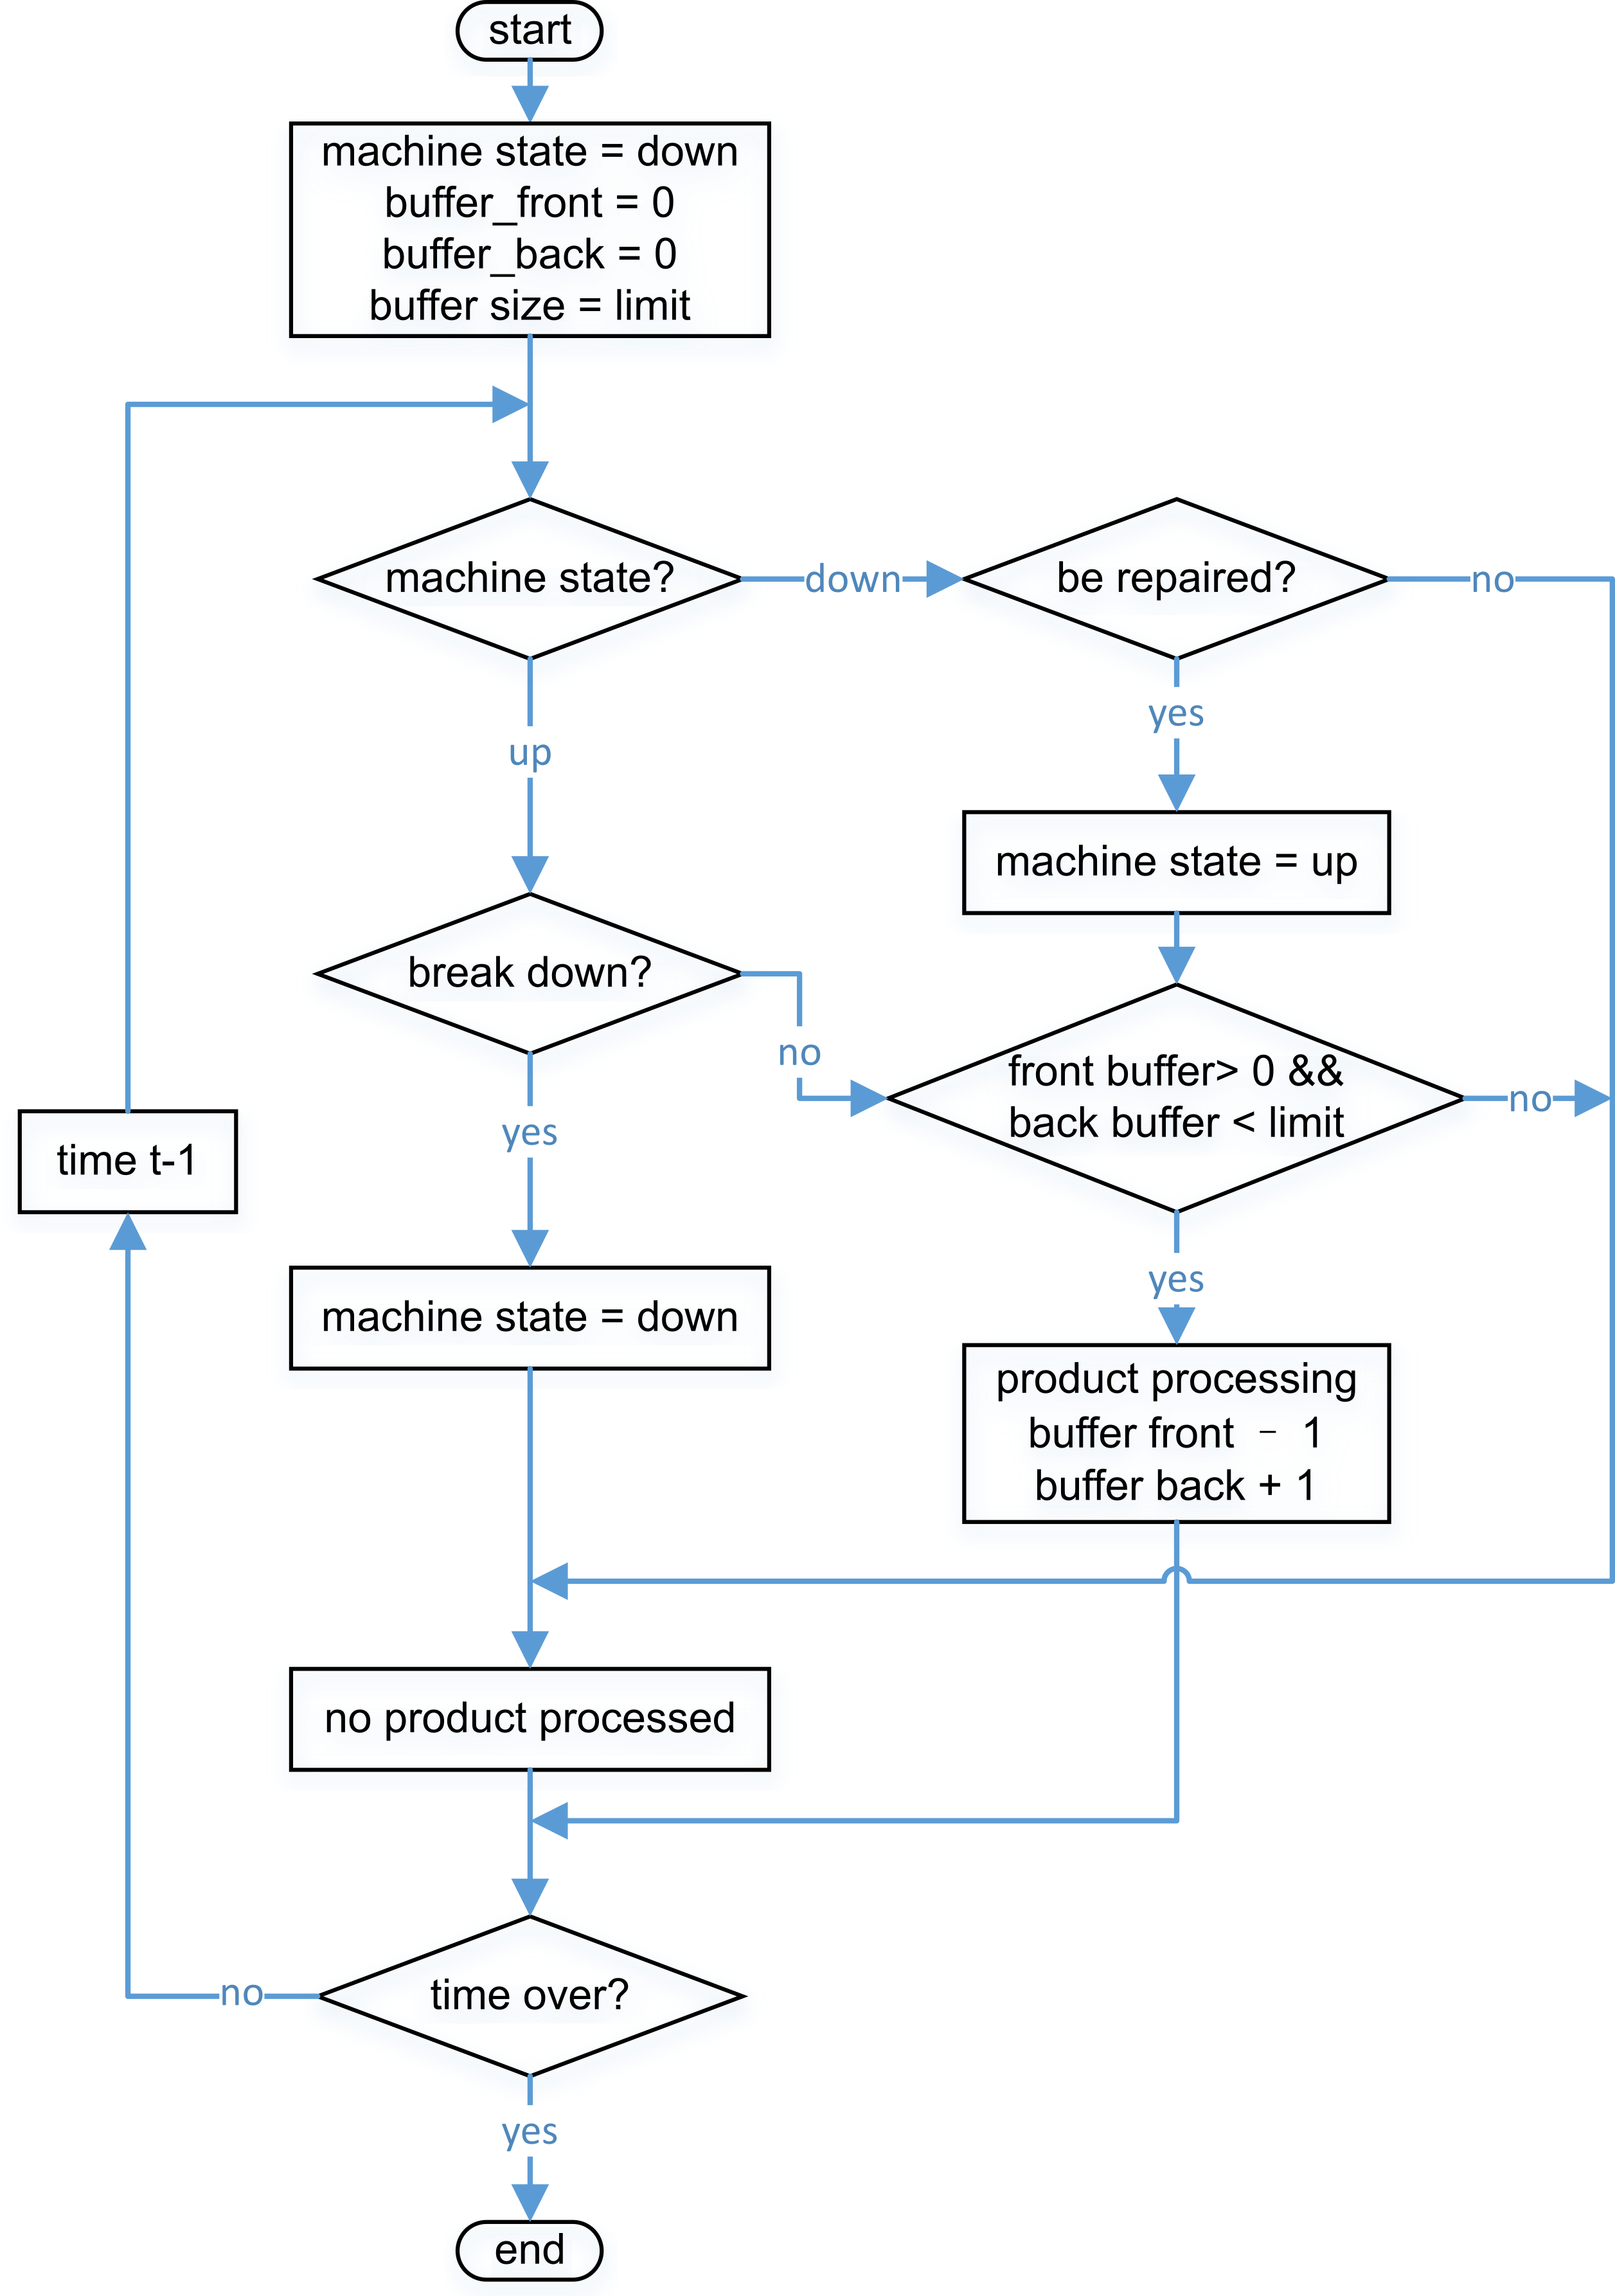
\includegraphics[width=0.62\linewidth]{procedure.png}	
	\caption{Flow chart of Procedure.}
    \label{flow chart}
\end{figure*}
\section{Procedure Description}
\noindent We suppose that a suitable buffer size can help to improve the transient performance of the production line. On the other hand, if the buffer size is designed . Therefore, we design a experiment on a five-machine production-line model. We use the following parameters:
\begin{displaymath}
    P = 0.05, R = 0.2, N = 1,...20, \text{All Buffer storage = epmty}
\end{displaymath}

In order to describe the procedure, we use a flow chart to illustrate the critical part of the program logic. At the beginning, we initialize all the parameters given in the file ''simulation.py''. Next, the parameters are passed to the file called ''multi\_machine.py'', and a certain amount of this object are created from the \pythoninline{class MultiMachine} to calculate the average of the cirtical values. Furthermore, the related machine objects and buffer objects will be created and simulated according to the procedure shown in flow chart. 

When the programm creates a simulated geomatric machine line, it first initiallize states of all machines and storages of all buffers. After that, in each time slot two conditional function will be called sequentially in order to make sure whether the machine break down , and if it can to be repaired or may break down according to its present state espectively. If the machine is in good condition (i.e. it can work), thereupon another conditional function will be called to test if the buffer in front of the machine has at least one product (except the first machine) or the buffer at the end of the machine has enough space to receive one new product (except the last machine). If all these conditions filling, then the machine produce a product, and at the same time take one product from the front buffer with put a product in the back buffer.

\section{Results and Discussion}
\noindent After the simulation, we collected the data of evaluation of transient performance of the geomatric machine lines. The Figure 1 shows with the buffer size enlarging the trend of the production rate. Figure 2 shows that this trend of 

\begin{figure*}[!h]
    \centering
    \subfigure[]{                
		\includegraphics[width=0.45\linewidth]{pr_n.tikz}	
    % \caption{Variance of Production Rate with N buffer size.}
    \label{pr buffer size}
    }
    \subfigure[]{
        \includegraphics[width=0.45\linewidth]{cr_n.tikz}
        % \caption{Variance of Consumption Rate with N buffer size.}
    \label{cr buffer size}
        }
    \caption{Variance of Transient Parameters. (a) Production Rate; (b) Consumption Rate.}
    \label{p c rate N buffer}
\end{figure*}